\subsection*{Social Media Storage Estimate:}
Social media sites seldom reveals the amount of data they store or ingest on a daily basis. Also the ever growing social media makes it hard to estimate their storage capacity. I present few methods in the following section to estimate the social media storage.

\Paragraph{1. Storage space estimate from media units:}
This method works for all the social media sites metioned in Table \ref{table:media_units} where the approximate storage space required by a media unit is known.

\paragraph{Youtube:}
Let us take an example of a Youtube video data. From Table  \ref{table:media_units}, we find that in the year 2017 users uploaded 720,000 hours of video on Youtube per day. First, assuming the fact that Youtube fairly stores most of the videos
 in 1080p and also stores them in multiple resolution such as 240p, 360p, 720p and format e.g. Webm, flv, mp4, 3gp, mp3. We can determine the amount of storage space needed for a 1 minute video \cite{youtube_stats}.

\begin{equation}
\begin{split}
  &27.71 \text{ MB (Webm)} + 17.00 \text{ MB (flv)} + 554.43 \text{ KB (3gp)} \\
  &+ 45.80 \text{ MB (mp4)} + 2.81 \text{ MB (mp3)}\\
  &= 93.8614355 \text{ MB}\\
  \end{split}
  \label{eq:youtube}
\end{equation}
 From the above Equation \ref{eq:youtube}, we find that $720,000 \times 60 \times 93.8614355 \approx 4.055$ petabytes (PB)  of storage space is required by Youtube everyday. We can also calculate the total amount of storage space ingested during the period of 2013 to 2017 from Table \ref{table:media_units} by utilizing area under the curve method with interpolation. The above method reckons 3096.17 PB or 3.096 exabytes (EB) of storage. Considering videos before 2013 and new 4K video which takes more space, it can be easily assumed that Youtube uses 10-15 EB of storage space.

\paragraph{Twitter:}
Similar to the method above, we can find the space required to store a tweet. A tweet is stored in Twitter as UTF-8 format. This takes 140 characters tweets atmost 560 bytes of space. However the metadata attached with a tweet is much more than the tweet itself. I personally did a random sample experiment of 100K tweets stord in our databases to find the average storage space for tweet json object obtained from streaming api. I found that one json tweet object takes 3247 bytes of space in average.
682 million tweets per day will require around 2.2145 terabytes of data per day. Using the interpolation method for area under the curve, we can find that Twitter uses 3.13 petabyte of space for storing the tweet alone. It is also worth noting that 42\% of tweets contains images \cite{tweets_images}. If we assume the average image size be 100 KB then we will see $(100 * 1024)/3247 * 42 \% \approx 13.2$ times increase in storage space requirement.

\begin{figure}[t]
	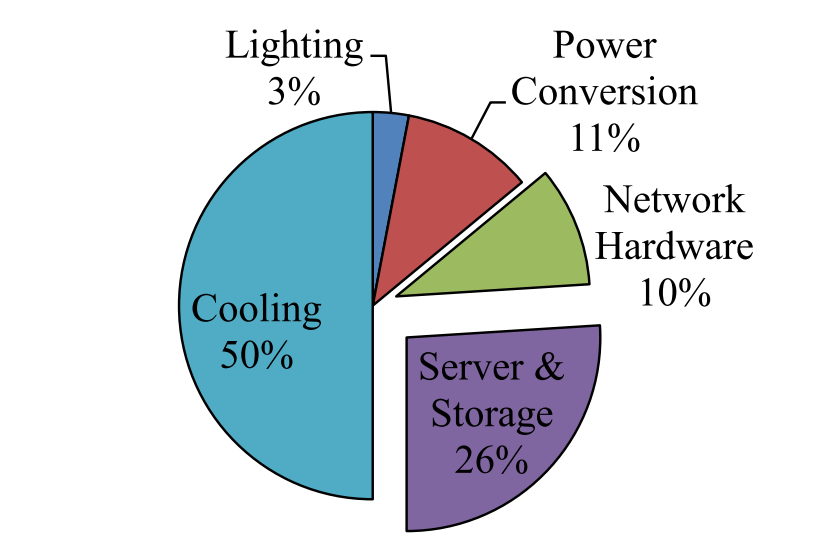
\includegraphics[width=0.7\linewidth ]{fig/energy_usage.png}
    \vspace{-2mm}
    \caption{A typical breakdown of energy usage among components in data center \cite{info2007top}.}
    \label{fig:energy_usage}
\end{figure}

\Paragraph{2. Storage space estimate from data center power usage:}
This section presents an approximate method to estimate space capacity of large social media companies like Facebook and Google.
A typical breakdown of energy consumption by data center is given in Figure \ref{fig:energy_usage}.
The largest energy consuming component is cooling infrastructure with 50\% of total energy. Rest of the energy is used by power conversion, lighting, network and server components \cite{info2007top, dayarathna2016data}. Facebook data centers use efficient data center architecture and hardware tweaks  saves
8-12\% of energy spent in cooling, 13-25\% in power conversion, 10\% in motherboard \cite{frachtenberg2011high}. That implies atmost 11\%  more efficient than typical data centers. Hence, it can be claimed that Facebook servers use 37\% of energy. Considering Facebook's 138 MW Altoona data center equipped with 200 Watts servers each with $6\times4$ TB of HDD as used in their experiment for \cite{frachtenberg2011high}. Assuming the datacenter is running at peak energy $(138 \times 0.37 \times 24)/ 200 = 6127200$  TB $= 6.1272$ exabytes (EB).
Taking all the data centers in consideration and diving them with replication factor we can estimate the storage capacity of Facebook. The analysis provided above supports news {\em Facebook Builds Exabyte Data Centers for Cold Storage} in 2013 \cite{facebook_support}.


\subsection*{Social Media Data for Researchers:}
Regardless of the vast data in social media sites, the dataset availables for researchers in public domain is very very limited. Also these datasets size are miniscule in comparison to what we mean by bigdata. The only exception is Twitter. Twitter provides $\tilde 1\%$ of sample tweets through its streaming API. By utilizing multiple resources and some other APIs such as keyword search researchers can obtain more than 1\% sample data. Also it is noteworthy to note that researchers looking for geotagged data faces a greater challenge as only 0.85\% of tweets in Twitter are geotagged \cite{sloan2013knowing}. A study on the sample tweets and orginial stream (firehose) reveals that the research on sample and original can differ unless proper coverage is taken care of during data collection strategy  \cite{morstatter2013sample}. From the previous analysis and checking our twitter streaming collection, we can estimate that $\tilde 1\%$ sample collects 25-30 GB of uncompressed data daily.

Facebook has tightened the security and restricted access to many of its data for public research after Cambridge Analytical Scandal \cite{cambridge_analytica, fb_data}. However, Facebook launched an initiative to make a dataset available to {\em ``The Social Science Research Council"} for assessment on impact of social data on elections \cite{fb_initiative}. That means only affiliated researchers with certain agencies will be able to access Facebook's data. I believe we will continue to see a restricted access behavior from similar social media sites in future which can affect public researchers.

To sum up, I present some of the most relevant social media dataset available for public research in Table \ref{table:datasets}. From Table \ref{table:datasets}, it is clear that there is no relationship between the amount of data social media sites possesses and the data available for researchers in public domain.

Many social media sites expose APIs for developers to access data. The free APIs of all the relevant social media sides are very restrictive. For example, facebook allows 200 api requests per hours/user. Instagram earlier had 5000 requests/hour which has been reduced to 200 request/hour. Geolocation services like foursquare 500 requests/hour on premium API end points. Hence, it is clear that the availability of social media data in public domain is not only subjected to efforts we invest in collecting it but also restrictive policies from companies. We will revisit about {\em scraping challanges} in the next section.

\begin{table}[t]
  \vspace{5mm}
      \caption{Most relevant social media dataset. }
      \vspace{-3mm}
{\small
\centering
    \begin{adjustbox}{width=1.05\linewidth,center}
\begin{tabular}{|l | l | r | l |} \hline
   \textbf{Site}                         & \textbf{Dataset}     & \textbf{Size} & \textbf{Link}  \\ \hline

   \multirow{5}{*}{\begin{tabular}{@{}l@{}} \href{http://networkrepository.com/}{Network Repository} \end{tabular}} &    Frienster      & \multicolumn{1}{r|}{8 GB} &  \href{http://networkrepository.com/soc-friendster.php}{link}   \\  \cline{2-4}

               & Twitter (1)      & \multicolumn{1}{r|}{6 GB} &  \href{http://networkrepository.com/soc-twitter-mpi-sws.php}{link}  \\\cline{2-4}

               & Twitter (2)      & \multicolumn{1}{r|}{6 GB} &  \href{http://networkrepository.com/soc-twitter.php}{link}  \\\cline{2-4}

               & Twitter (3)      & \multicolumn{1}{r|}{960 MB} &  \href{http://networkrepository.com/soc-twitter-2010.php}{link}  \\\cline{2-4}

               & Orkut (1)     & \multicolumn{1}{r|}{388 MB} &  \href{http://networkrepository.com/soc-orkut.php}{link}  \\\cline{2-4}

               & Orkut (2)     & \multicolumn{1}{r|}{422 MB} &  \href{http://networkrepository.com/soc-orkut-dir.php}{link}  \\\cline{2-4}


               & Sina Weibo      & \multicolumn{1}{r|}{960 MB} &  \href{http://networkrepository.com/soc-sinaweibo.php}{link}  \\\cline{1-4}

     \multirow{5}{*}{\begin{tabular}{@{}l@{}} \href{https://snap.stanford.edu/data/}{Stanford SNAP} \end{tabular}} &    Facebook (ego)      & \multicolumn{1}{r|}{4,039 nodes} &  \href{http://snap.stanford.edu/data/ego-Facebook.html}{link}   \\  \cline{2-4}

                 & Google Plus      & \multicolumn{1}{r|}{107,614 nodes} &  \href{http://snap.stanford.edu/data/ego-Gplus.html}{link}  \\\cline{2-4}

                 & Twitter Social      & \multicolumn{1}{r|}{81,306 nodes} &  \href{http://snap.stanford.edu/data/ego-Twitter.html}{link}  \\\cline{2-4}

                 & Expinion      & \multicolumn{1}{r|}{75,879 nodes} &  \href{http://snap.stanford.edu/data/soc-Epinions1.html}{link}  \\\cline{2-4}

                 & Youtube     & \multicolumn{1}{r|}{1,134,890 nodes} &  \href{http://snap.stanford.edu/data/com-Youtube.html}{link}  \\\cline{2-4}

                 & Amazon Product     & \multicolumn{1}{r|}{334,863	 nodes} &  \href{http://snap.stanford.edu/data/com-Amazon.html}{link}  \\\cline{2-4}

                 & Reddit     & \multicolumn{1}{r|}{132,308 submissions} &  \href{http://snap.stanford.edu/data/web-Reddit.html}{link}  \\\cline{2-4}

                & Flickr     & \multicolumn{1}{r|}{2,316,948 images} &  \href{http://snap.stanford.edu/data/web-flickr.html}{link}  \\\cline{2-4}


                & BrightKite (Location)     & \multicolumn{1}{r|}{58,228 Nodes} &  \href{http://snap.stanford.edu/data/loc-Brightkite.html}{link}  \\\cline{2-4}

                 & Gowalla (Location)     & \multicolumn{1}{r|}{196,591 Nodes} &  \href{http://snap.stanford.edu/data/loc-Gowalla.html}{link}  \\\cline{2-4}

                 & Movies & \multicolumn{1}{r|}{196,591 Nodes} &  \href{http://snap.stanford.edu/data/web-Movies.html}{link} \\\cline{1-4}

     \multirow{5}{*}{\begin{tabular}{@{}l@{}} \href{http://socialcomputing.asu.edu/pages/datasets}{Social Computing ASU} \end{tabular}} &    Youtube (1)      & \multicolumn{1}{r|}{1,138,499 nodes} &  \href{http://socialcomputing.asu.edu/datasets/YouTube2}{link}   \\  \cline{2-4}

                 & Youtube (2)      & \multicolumn{1}{r|}{15088 nodes} &  \href{http://socialcomputing.asu.edu/datasets/YouTube}{link}  \\\cline{2-4}

                 & Last FM      & \multicolumn{1}{r|}{108,493 nodes} &  \href{http://socialcomputing.asu.edu/datasets/Last.fm}{link}  \\\cline{2-4}

                 & Twitter      & \multicolumn{1}{r|}{11,316,811 tweets} &  \href{http://socialcomputing.asu.edu/datasets/Twitter}{link}  \\\cline{2-4}

                 & Flickr      & \multicolumn{1}{r|}{80,513 nodes} &  \href{http://socialcomputing.asu.edu/datasets/Flickr}{link}  \\\cline{2-4}

                 & Foursquare     & \multicolumn{1}{r|}{106,218 nodes} &  \href{http://socialcomputing.asu.edu/datasets/Foursquare}{link}  \\\cline{2-4}

                 & Digg      & \multicolumn{1}{r|}{116,893 nodes} &  \href{http://socialcomputing.asu.edu/datasets/Digg}{link}  \\\cline{2-4}


                 & Delicious      & \multicolumn{1}{r|}{103,144 nodes} &  \href{http://socialcomputing.asu.edu/datasets/Delicious}{link}  \\\cline{1-4}

       \multirow{1}{*}{\begin{tabular}{@{}l@{}} \href{http://help.sentiment140.com/for-students}{Sentiment  140} \end{tabular}} &    Twitter Sentiment      & \multicolumn{1}{r|}{160,000 tweets} &  \href{http://help.sentiment140.com/for-students}{link}   \\  \cline{1-4}

       \multirow{1}{*}{\begin{tabular}{@{}l@{}} \href{https://www.reddit.com/r/datasets/comments/3bxlg7/i_have_every_publicly_available_reddit_comment/}{Reddit } \end{tabular}} &    Reddit     & \multicolumn{1}{r|}{1.7 billion comments} &  \href{https://www.kaggle.com/reddit/reddit-comments-may-2015}{link}   \\  \cline{1-4}

       \multirow{1}{*}{\begin{tabular}{@{}l@{}} \href{https://www.reddit.com/r/datasets/comments/3bxlg7/i_have_every_publicly_available_reddit_comment/}{Yahoo} \end{tabular}} &    Flickr      & \multicolumn{1}{r|}{100 million images} &  \href{ https://yahooresearch.tumblr.com/post/89783581601/one-hundred-million-creative-commons-flickr-images}{link}   \\  \cline{1-4}

        \multirow{2}{*}{\begin{tabular}{@{}l@{}} \href{}{Awesome Data Github} \end{tabular}} &    Google Scholar      & \multicolumn{1}{r|}{Unknown} &  \href{ http://www3.cs.stonybrook.edu/~leman/data/gscholar.db}{link}   \\  \cline{2-4}

          & Indie Map      & \multicolumn{1}{r|}{Unknown} &  \href{http://www.indiemap.org/}{link}  \\\cline{1-4}


 \end{tabular}
 \end{adjustbox}
 % \vspace{ + 15 mm}
 }
 \label{table:datasets}
 \end{table}




%%% Local Variables:
%%% mode: latex
%%% TeX-master: "main"
%%% End:
